%%%%%%%%%%%%%%%%%%%%%%%%%%%%%%%%%%%%%%%%%%%%%%%%%%%%%%%%%%%%%%%%%%%%%%
% How to use writeLaTeX: 
%
% You edit the source code here on the left, and the preview on the
% right shows you the result within a few seconds.
%
% Bookmark this page and share the URL with your co-authors. They can
% edit at the same time!
%
% You can upload figures, bibliographies, custom classes and
% styles using the files menu.
%
%%%%%%%%%%%%%%%%%%%%%%%%%%%%%%%%%%%%%%%%%%%%%%%%%%%%%%%%%%%%%%%%%%%%%%

\documentclass[12pt]{article}

\usepackage{sbc-template}

\usepackage{graphicx,url}

\usepackage[T1]{fontenc}
%\usepackage[brazil]{babel}   
\usepackage[utf8]{inputenc}  

\usepackage{float}

     
\sloppy

\title{Avaliação de Desempenho de Roteadores}

\author{André Hoffmann\inst{1}, Bruno Vieira\inst{1},Christian Lima\inst{1}, Gian Boschetti\inst{1},\\Jéferson Bueno\inst{1} e Rafael Christ\inst{1} }


\address{Curso de Bacharelado em Ciência da Computação \\Universidade do Vale dos Sinos (UNISINOS) – Campus de São Leopoldo \\
+55 (51) 3591-1122 – São Leopoldo – RS– Brasil 
  \email{\{andresh,brunopv,christianml,gianboschetti,jsbueno,rschrist\}@edu.unisinos.br}
}

\begin{document} 

\maketitle

\begin{abstract}
  This article describes the performance evaluation of a router in two distinct scenarios: with the router and without the router. The goal is determine the actual performance of the router and observe how it varies according to the size of the datagram. After the performance evaluation, it was possible to verify that there was no relevant byte or packet throughput variation between the scenarios, however, it was possible to notice an increase in CPU usage as the packets decrease in size.
\end{abstract}
     
\begin{resumo} 
  Este artigo descreve a avaliação de desempenho de um roteador em dois cenários distintos: com o roteador e sem o roteador. O objetivo é determinar o real desempenho do roteador e observar se como ele varia de acordo com o tamanho do datagrama. Após a avaliação de desempenho, foi possível constatar que não houve variação de vazão de bytes ou pacotes relevante entre os cenários, no entanto, foi possível notar um aumento no uso de CPU conforme os pacotes diminuem de tamanho.
\end{resumo}


\section{Introdução}

Nos dias de hoje roteadores são um dos equipamentos mais utilizados no compartilhamento de rede, seja em ambientes corporativos ou ambientes residenciais. Existem diversos modelos e marcas no mercado, assim como diferentes especificações técnicas para estes modelos de roteadores. Em muitos casos, o uso de um roteador não se faz necessário para realizar a conexão entre dois computadores, entretanto, fabricantes tem se esforçado constantemente para que o uso do mesmo não prejudique o desempenho final da conexão e, em alguns casos, tenha até mesmo o desempenho aprimorado. Desta forma, é importante medirmos o desempenho de dispositivos que utilizamos, a fim de detectar qualquer tipo de lesão aplicada ao usuário por parte da fabricante.

Este trabalho tem como objetivo apresentar a avaliação de desempenho de um roteador, obervando se e como ele varia, de acordo com o tamanho do datagrama enviado. Este artigo procura responder o que é a avaliação de desempenho, qual sua importância, qual o comportamento do roteador em relação ao tamanho dos datagramas e se as fabricantes falam a verdade com relação ao desempenho de seus roteadores.


\section{Avaliação de desempenho}

Esta seção detalha a definição da metodologia de avaliação de desempenho, assim como a descrição dos cenários aplicados.

\subsection{Metodologia de avaliação de desempenho}
De acordo com Farias (2008), "avaliar um sistema é pronunciar-se sobre as características do mesmo, ou seja, é realizar toda
e qualquer observação sobre o mesmo. Com isso existem basicamente dois tipos de avaliação,
qualitativa e quantitativa. Na avaliação qualitativa, existe a necessidade de uma comparação com
o senso comum ou com valores de referência. A avaliação quantitativa baseia-se na formulação
de valores específicos sem levar em consideração os méritos dos valores obtidos".

Podemos considerar que toda avaliação de desempenho busca um julgamento qualitativo, contudo, toda avaliação científica é feita com base em resultados quantitativos.

Segundo Pidd (1992), existem três técnicas de avaliação de desempenho: Monitoração, Simulação e Métodos Analíticos.
A monitoração contempla a observação de sistemas reais, proporcionando uma maior fidelidade quanto aos resultados obtidos.
Esta técnica, contudo, geralmente possui custo e tempo de análise elevados. A simulação propõe a construção de um modelo para simular o funcionamento do sistema em questão, descrevendo características funcionais do sistema em uma escala adequada. Apesar desta técnica conter detalhes importantes do sistema, possui um certo nível de abstração.
Métodos analíticos são, assim como a simulação, baseados em um modelo do sistema real, contudo, possuem um nível de abstração muito maior, pois o modelo é puramente matemático.
Para este trabalho, a avaliação de desempenho foi realizada de maneira quantitativa e utilizando a técnica de simulação.

\subsection{Cenários aplicados}

Conforme a especificação para avaliação a ser aplicada neste trabalho, o teste a ser realizado consiste na transmissão de uma série de pacotes, com diferentes tamanhos (128, 256, 512, 1024 e 1280 bytes), de um micro A (em modo servidor) para um micro B (em modo cliente), transmitidos via protocolo UDP, utilizando o programa IPERF. Estas transmissões foram realizados cerca de 10 vezes para cada tamanho de pacote, por 30 segundos em cada vez. Cada teste foi realizado em duas faixas de largura de banda (80\%, equivalente a 80Mb/s e 100\%, equivalente a 100Mb/s)

Estes testes foram realizados em dois cenários distintos, descritos a seguir:

\begin{figure}[ht]
\centering
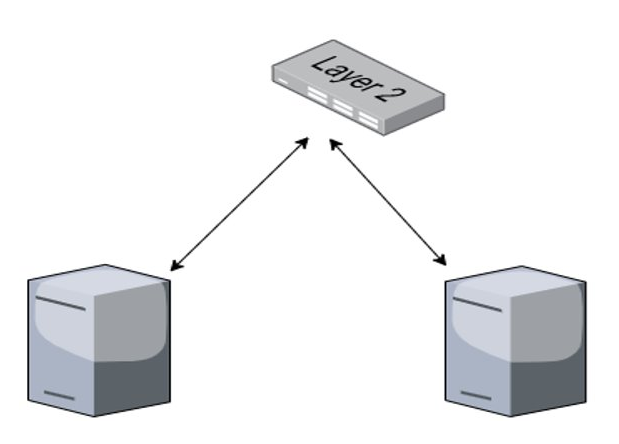
\includegraphics[width=.5\textwidth]{fig_sem_roteador.png}
\caption{Cenário 1}
\label{fig:fig_sem_roteador}
\end{figure}

\subsubsection{Cenário 1}

Neste cenário a conexão proposta entre os dois computadores é realizada sem utilizar um roteador, ou seja, interligados diretamente. Entretanto, não foi possível obter um cabo crossover para os testes, desta forma, ambos computadores foram conectados em um switch gigabit ethernet, conforme a Figura 1.

\subsubsection{Cenário 2}

\begin{figure}[ht]
\centering
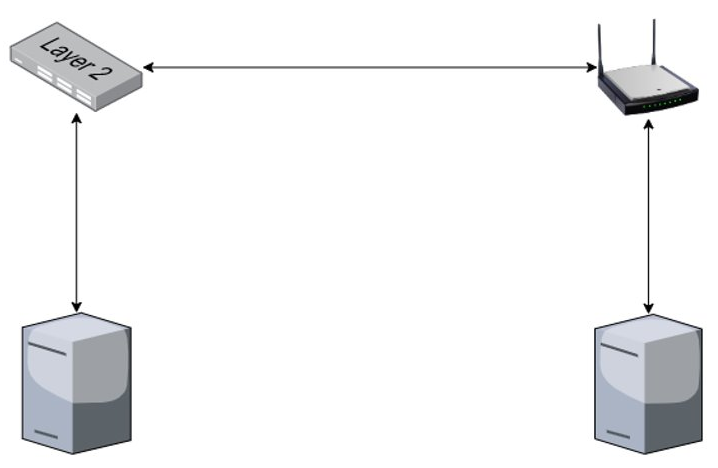
\includegraphics[width=.5\textwidth]{fig_com_roteador.png}
\caption{Cenário 2}
\label{fig:fig_com_roteador}
\end{figure}

Neste cenário a conexão proposta entre os dois computadores é realizada com o intermédio de um roteador. Contudo, como há o uso de um switch no Cenário 1, o uso do mesmo também foi aplicado neste cenário, com objetivo de causar o mínimo de interferência no comparativo dos testes.
A figura 2 exemplifica a conexão do Cenário 2.

\subsubsection{Comandos IPERF}

Os comandos utilizados no IPERF para a realização do teste possuem o seguinte padrão:
\newline
\newline
\textbf{Servidor:}
\newline
\texttt{iperf --server --port 9000 --udp --len <TAMANHO\_DATAGRAMA>}
\newline
\newline
\textbf{Cliente:}
\newline
\texttt{iperf --format m --interval 1 --time 30 --client <IP\_SERVIDOR> --port 9000 --udp --bandwidth <LARGURA\_DE\_BANDA> --len <TAMANHO\_DATAGRAMA>}
\newline

Sendo <TAMANHO\_DATAGRAMA> o tamanho do datagrama, <IP\_SERVIDOR> o IP do servidor e <LARGURA\_DE\_BANDA> a largura de aplicada.

\subsection{Resultados esperados}

Para cada largura de banda em cada cenário, tem-se por objetivo a obtenção dos seguintes resultados:

\subsubsection{Vazão de pacodes na rede}

A vazão de pacotes é definida como o número de pacotes que podem ser transmitidos sobre a rede num dado tempo.

\subsubsection{Vazão de bytes na rede}

A vazão de pacotes é definida como o número de bytes que podem ser transmitidos sobre a rede num dado tempo.

\subsubsection{Utilização da CPU}

Consiste no uso de CPU utilizado durante a transmissão.

\section{Equipamentos utilizados}

Esta seção detalha quais equipamentos foram utilizados na avaliação de desempenho.

\subsection{Micro A}

Desktop utilizado como servidor do IPERF. Conta com processador AMD Ryzen 7 1700, com 8 cores e 16 threads; memória RAM DDR4 de 16 GB; controladora de rede Intel I211-AT Gigabit Ethernet e sistema operacional Ubuntu 19.10 (Linux). 

\subsection{Micro A}

Desktop utilizado como servidor do IPERF. Conta com processador AMD Ryzen 7 1700, com 8 cores e 16 threads; memória RAM DDR4 de 16 GB; controladora de rede Intel I211-AT Gigabit Ethernet e sistema operacional Ubuntu 19.10 (Linux). 

\subsection{Micro B}

Notebook utilizado como cliente do IPERF. Possui processador Intel Core i7 4500U, com 2 cores e 4 threads; memória RAM DDR3 de 8 GB; controladora de rede Realtek PCIe Fast-Ethernet e sistema operacional Ubuntu 19.10 (Linux) 

\subsection{Switch}

Switch não-gerenciável (sem sistema operacional próprio e de operação simplificada), que interconecta ambos os equipamentos acima listados. O Switch utilizado nos testes conta com interfaces de rede Gigabit Ethernet. A fabricante desse é TL-SG108 não gerenciável. 

\subsection{Roteador}

O Roteador utilizado para testes específicos do cenário 2 consta com interfaces de fast ethernet. Uma interface de rede com Fast Ethernet (também conhecida como 10/100), consegue transferir dados em taxas de até 100 Megabit por segundo. O modelo e marca do roteador utilizado são D-Link e DIR-615, respectivamente.

\subsection{Cabos de rede}

Os cabos utilizados nos cenários de teste utilizam a tecnologia CAT5e, tecnologia essa denominada como uma versão melhor do CAT5, esta tecnologia possui maior proteção à interferência externa, tendo em vista que os testes não possuem influências externas, o Cat-5e é mais do que suficiente para o teste.

\section{Resultados obtidos}

Esta seção detalha os resultados obtidos na avaliação de desempenho.

\subsection{Vazão de pacotes na rede}

\begin{figure}[H]
\centering
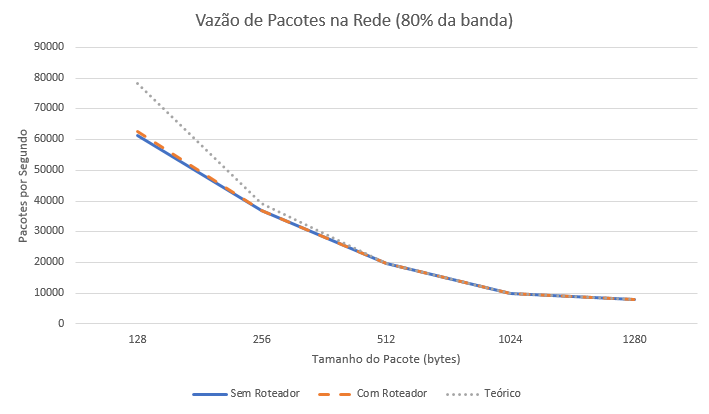
\includegraphics[width=.9\textwidth]{vazao_pac_80.png}
\caption{Vazão de pacotes (80\% de banda)}
\label{fig:fig_com_roteador}
\end{figure}

A Figura 3 apresenta o gráfico da vazão de pacotes na rede com a utilização de 80\% da banda, no eixo vertical, temos a informação da quantidade de pacotes por segundo. Já no eixo horizontal, temos o tamanho do pacote, medido em bytes.

\begin{figure}[H]
\centering
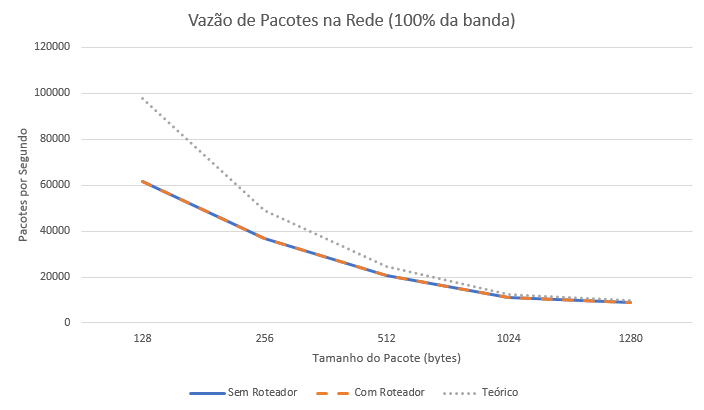
\includegraphics[width=.9\textwidth]{vazao_pac_100.png}
\caption{Vazão de pacotes (100\% de banda)}
\label{fig:fig_com_roteador}
\end{figure}

A Figura 4 possui estrutura semelhante, desta vez apresentando os dados com base no uso de 100\% da banda.

\subsection{Vazão de bytes na rede}

\begin{figure}[H]
\centering
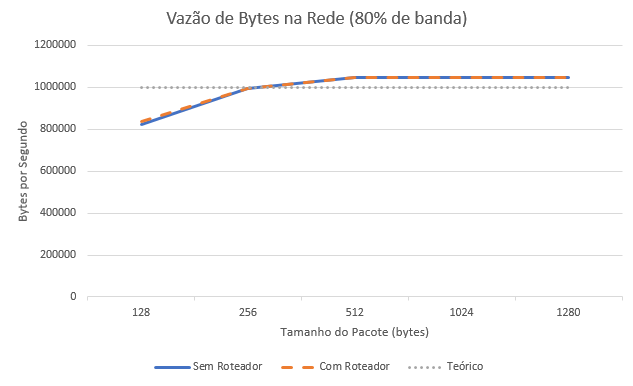
\includegraphics[width=.9\textwidth]{vazao_bytes_80.png}
\caption{Vazão de bytes (80\% de banda)}
\label{fig:fig_com_roteador}
\end{figure}

A Figura 5 apresenta o gráfico da vazão de bytes na rede com a utilização de 80\% da banda, no eixo vertical, temos a informação da quantidade de bytes por segundo. Já no eixo horizontal, temos o tamanho do pacote, medido em bytes.

\begin{figure}[H]
\centering
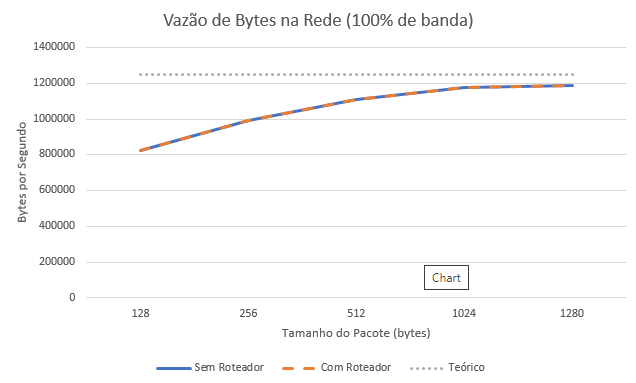
\includegraphics[width=.9\textwidth]{vazao_bytes_100.png}
\caption{Vazão de bytes (100\% de banda)}
\label{fig:fig_com_roteador}
\end{figure}

A Figura 6 possui estrutura semelhante, desta vez apresentando os dados com base no uso de 100\% da banda.

\subsection{Utilização de CPU}

\begin{figure}[ht]
\centering
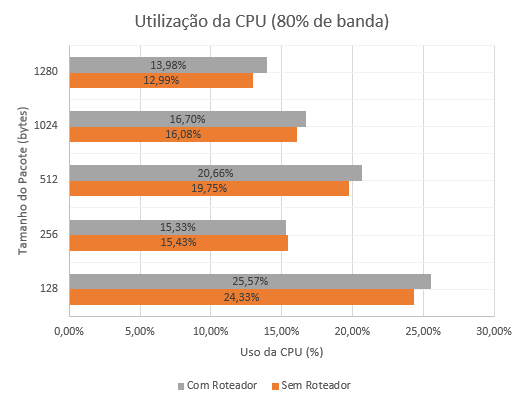
\includegraphics[width=.9\textwidth]{uso_cpu_80.png}
\caption{Uso de CPU (80\% de banda)}
\label{fig:fig_com_roteador}
\end{figure}

A Figura 7 apresenta o gráfico da utilização da CPU com base no uso de 80\% da banda, no eixo vertical, temos a informação do tamanho do pacote. Já no eixo horizontal, temos o percentual de uso da CPU.

\begin{figure}[H]
\centering
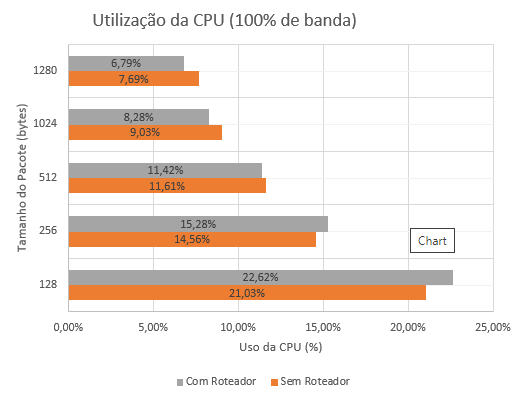
\includegraphics[width=.9\textwidth]{uso_cpu_100.png}
\caption{Uso de CPU (100\% de banda)}
\label{fig:fig_com_roteador}
\end{figure}

A Figura 8 possui estrutura semelhante, desta vez apresentando os dados com base no uso de 100\% da banda.

\section{Conclusão}

Ao final dos testes e obtenção dos resultados da avaliação de desempenho foi possível constatar que tanto a vazão de bytes quanto a vazão de pacotes não apresentaram diferença significativa entre os cenários, independentemente do tamanho de pacote utilizado. 
Especula-se que isto tenha ocorrido devido à qualidade satisfatória do roteador, que não representa um  \textit{bottleneck} (gargalo) na comunicação em rede. Existe, ainda, o fato de que os testes realizados não possuem confiabilidade absoluta: todo o controle de transferências, largura de banda e afins foi realizado via software, ou seja, na camada de Aplicação, e está sujeito à influência de fatores externos como o sistema operacional, a controladora de rede, ou ainda o próprio meio de tráfego utilizado.
Quanto a utilização da CPU, foi possível notar que ocorre um aumento da mesma, conforme a diminuição de tamanho do datagrama enviado e, na maioria dos casos, o uso de CPU é maior com o uso do roteador.

\section{Referências}

Bolla, Raffaele, and Roberto Bruschi. "Linux software router: data plane optimization and performance evaluation." Journal of Networks 2.3 (2007): 6-17.

FARIAS, M. M.. Protocolo de roteamento para redes wireless mesh. Porto Alegre, 2008. Disponível em: <http://tede2.pucrs.br/tede2/handle/tede/5112> . Acesso em: 27 de abril de 2020.

https://iperf.fr/ - Acessado em: 12 de abril de 2020.

M. Pidd, Computer Simulation in Management Science, 3rd ed., I. John Wiley \& Sons, Ed. New York, NY, USA: John Wiley \& Sons, Inc., 1992.

VERGANI, Lazaro. Saiba as diferenças entre cabos CAT5, CAT5e, CAT6, CAT7 e CAT8. 2017. Disponível em: <https://www.onixsecurity.com.br/blog/saiba-as-diferencas-entre-cabo-cat5-cat5e-e-cat6/>. Acesso em: 27 de abril de 2020

%\bibliographystyle{sbc}
%\bibliography{sbc-template}

\end{document}
